\documentclass[12pt,a4paper]{article}
\usepackage[latin1]{inputenc}
\usepackage{amsmath}
\usepackage{amsfonts}
\usepackage{amssymb}
\usepackage{graphicx}
\author{Jeremy Scheurer}
\title{Intuition about Vector Calculus}

% The content provided in this document is all taken from the website mathinsight.org and was solely summarized for private usage.

\begin{document}
	\section{Line Integral of scalar-valued functions}
	
	\begin{itemize}
	
	\item The idea is similar to the one of an Integral over a two dimensioal Surface. As analogy you can imagine to calculate the mass of a wire from its density. 
	
	\item Assume you have a wire whose density is not constant over its length. We have a function $C(t)$ which describes a certain point on the wire. How can you calcuate it's mass from its density?
	
	\item We can segment the wire into lots of smaller segments and calculate their mass according to the specific densities. The length of the i-th segment is defined as: $||c(t_i) - c(t_i -1)||$. \\
	The densitiy for a specific point is defined as: $f(c(t_i))$
	
	\item The mass of a segment is just the Linesegment $\cdot$ its density: \\
	$f(c(t_i))\cdot||c(t_i) - c(t_i -1)||$ \\
	To calculate the total mass of the whole wire you just have to sum up all the masses of the segments: $\sum_{i}^{n} f(c(t_i))\cdot||c(t_i) - c(t_i -1)||$
	
	\item To turn this into an integral we define: $ \Delta t_i = t_i - t_{i-1}$. Now multiply and divide each term by $\Delta t_i$ and obtain the more complicated looking expression: \\
	$\sum_{i}^{n} f(c(t_i))\cdot ||c(t_i)-c(t_{i-1})|| = \sum_{i}^{n}     ||\frac{c(t_{i-1} + \Delta t_i)-c(t_{i-1})}{\Delta t_i}|| \cdot \Delta t_{i-1}$
	
	\item You realize, that the term in the expression $||.||$ is actually the definition of the derivate off $c(t)$. The counter is nothing else than a function c(t) applied to an interval and the denominator is that exact interval. So if you apply it to a two-dimensional function it's nothing else than $\frac{\Delta y}{Delta x}$ which defines the secant. 
	
	For comparison here is the definition of the definition of a Secant: \\
	$\frac{f(x_0 + \Delta x) - f(x_0)}{\Delta x}$


	\item If we let $\Delta t_i \rightarrow 0$ and $n \rightarrow \infty $ the above Riemann sum converges to the integral:
	$\int_{a}^{b} f(c(t))\cdot ||c'(t)|| dt$ which is often denoted as $\int_{c}^{}f ds$.
	\end{itemize}
	
	\section{Introduction to a line integral of a vector field}
	
	\begin{itemize}
	\item The only change to the chapter above is that now we want to integrate a vector valued curve function along a curve. They are usually represented by a vector field. \\ $\textit{A very easy interpretation is to imagine the amount of work that a foce field does on a particle as it moves along a curve.}$
	
	\item 
	
	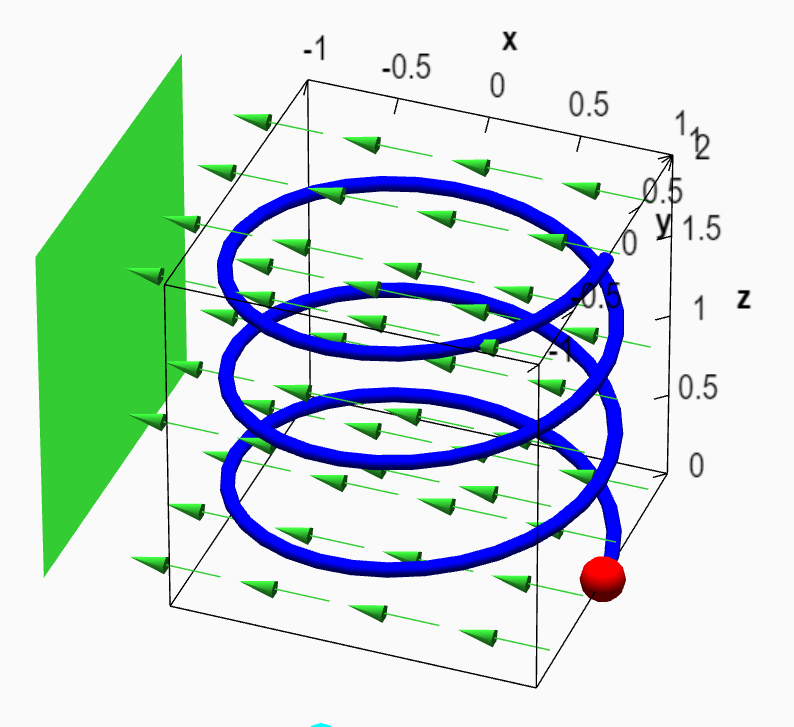
\includegraphics[width=0.7\textwidth, height = 30px]{C:\Users\jerem\Pictures\Screenshots\Field_Helix}
	\end{itemize}
	
	

\end{document}